\section*{贝叶斯网络}

\begin{frame}
\centerline{\textbf{\Large{贝叶斯网络}}} 
~\\
\centerline{\large{邵逸岚}}
\end{frame}

\subsection*{贝叶斯定理}
\begin{frame}
	\textbf{贝叶斯公式:}
	~\\
	\centerline{{\large $P(A|B)=\frac{P(B|A)P(A)}{P(B)}$}}
	~\\
	~\\
	~\\
	后验概率=(相似度*先验概率)/标准化常量 
\end{frame}

\subsection*{定义}
\begin{frame}
	贝叶斯网络(Bayesian Network)是一种经典的概率图模型,它借助有向无环图(Directed Acyclic Graph, DAG)来刻画属性之间的依赖关系,并使用条件概率表(Conditional Probability Table, CPT)来描述属性的\textbf{联合}概率分布。
\end{frame}

\subsection*{结构}
\begin{frame}
	\begin{figure}
		\centering
		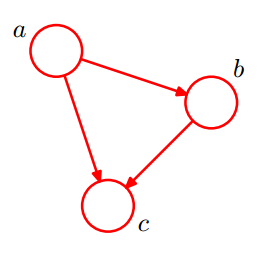
\includegraphics[scale=0.5]{pic/bn.png}
		\caption{贝叶斯网络结构图}
		\label{0-002}
	\end{figure}
\end{frame}

\begin{frame}
	贝叶斯网络B由结构G和参数$\Theta$构成,即$B=\langle G, \Theta\rangle$。给定父结点集,假设每个属性与它的非后裔属性独立,于是将属性$x_1, x_2, ..., x_d$的联合概率分布定义为:
	~\\
	~\\
	\centerline{{\large $P_B(x_1,x_2,...,x_d)=\prod_{i=1}^{d}P_B(x_i|\pi_i)=\prod_{i=1}^{d}\theta_{x_i|\pi_i}$}}
	~\\
	~\\
	以\ref{0-002}中的网络结构为例,联合概率分布可定义为:
	~\\
	~\\
	\centerline{{\large $P(a,b,c)=P(a)P(b|a)P(c|a,b)$}}
\end{frame}

\begin{frame}
\begin{figure}
	\centering
	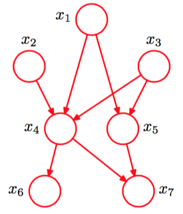
\includegraphics[scale=0.7]{pic/bayesian.png}
	\caption{较复杂的贝叶斯网络}
	\label{0-003}
\end{figure}
\end{frame}

\begin{frame}
	其联合概率分布可定义为:
	~\\
	~\\
	$P(x_1,...,x_7)=P(x_1)P(x_2)P(x_3)P(x_4|x_1,x_2,x_3)$
	\centerline{$\qquad\qquad p(x_5|x_2,x_3)P(x_6|x_4)P(x_7|x_4,x_5)$}
\end{frame}
	
\begin{frame}
	\begin{figure}
		\centering
		\begin{tabular}{ccc}
			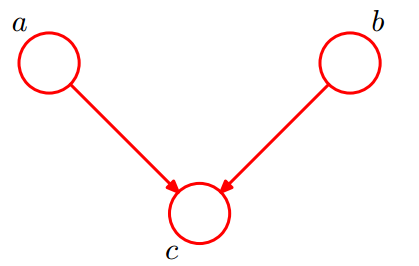
\includegraphics[width=0.28\linewidth]{pic/head2head.png} &
			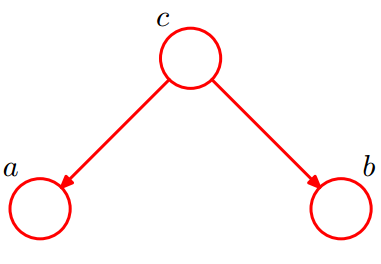
\includegraphics[width=0.28\linewidth]{pic/tail2tail.png} &
			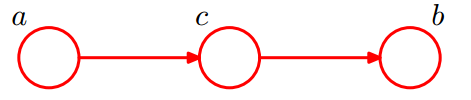
\includegraphics[width=0.28\linewidth]{pic/head2tail.png}\\
			(a) & (b) & (c) \\
			~\\
		\end{tabular}
		\caption{贝叶斯网络中属性的典型依赖关系}
		\label{0-004}
		\vspace{-0.5em}
	\end{figure}
\end{frame}

\begin{frame}
	(a)$\sum_{c}P(a,b,c)=\sum_{c}P(a)P(b)P(c|a,b)$ \\ $\Rightarrow P(a,b)=P(a)P(b)$
	~\\
	~\\
	(b)$P(a,b,c)=P(c)P(a|c)P(b|c)$ \\ $\Rightarrow P(a,b|c)=P(a|c)P(b|c)$
	~\\
	~\\
	(c)$P(a,b|c)=P(a,b,c)/P(c)$ \\ $\qquad\qquad\quad=P(a)P(c|a)P(b|c)/P(c)$ \\ $\qquad\qquad\quad=P(a,c)P(b|c)/P(c)$ \\ $\qquad\qquad\quad=P(a|c)P(b|c)$
\end{frame}

\subsection*{应用实例}
\begin{frame}
\begin{figure}
		\centering
		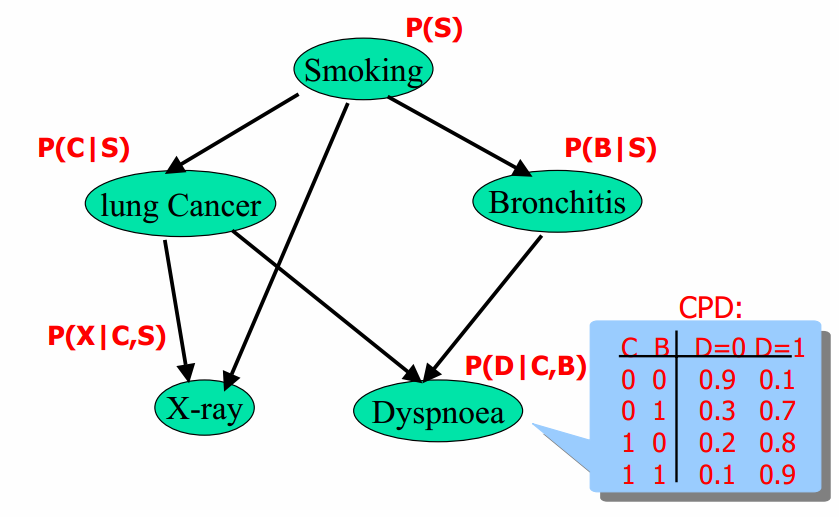
\includegraphics[scale=0.3]{pic/instance.png}
		\caption{贝叶斯网络实例}
		\label{0-005}
\end{figure}
\end{frame}

\subsection*{马尔科夫链}
\begin{frame}
	在给定$x_i$的条件下,$x_{i+1}$的分布与$x_1,x_2,...,x_{i-1}$无关,即$x_{i+1}$的分布只与$x_i$有关。这种顺次演变的随机过程,叫做马尔科夫链。马尔科夫链是贝叶斯网络的一种特例。
	~\\
	~\\
	\begin{figure}
		\centering
		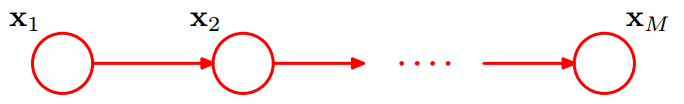
\includegraphics[scale=0.4]{pic/markov.png}
		\caption{马尔科夫链结构}
		\label{0-006}
	\end{figure}
\end{frame}

\begin{frame}
	马尔科夫链可表示为:
	~\\
	~\\
	\centerline{{\large $P(X_{n+1}=x|X_0,X_1,...,X_n)=P(X_{n+1}=x|X_n)$}}
	~\\
	~\\
	随机变量$X_1,X_2...$取值范围的合集成为“状态空间”,$X_i$的值表示在时间i的状态。马尔科夫链是时间和状态都是离散的马尔科夫过程。
\end{frame}

\begin{frame}
	如果状态空间是有限的,则转移概率分布可以表示为一个具有(i,j)元素的矩阵,称之为“转移矩阵”$\mathbf{P}$:
	~\\
	~\\
	\centerline{$P_{ij}=P(X_{n+1}=i|X_n=j)$}
	~\\
	对于一个离散状态空间,k步转移概率的积分即为求和,可以对转移矩阵求k次幂来求得。$\mathbf{P}^k$即是k步转移后的转移矩阵。\\平稳分布是一个满足以下方程的向量:
	~\\
	~\\
	\centerline{$\mathbf{P}\pi^*=\pi^*$}
	~\\
	在此情况下,稳态分布$\pi^*$是一个对应于特征根为1的、该转移矩阵的特征向量。
\end{frame}
